% 
% Annual Cognitive Science Conference
% Sample LaTeX Paper -- Proceedings Format
% 

% Original : Ashwin Ram (ashwin@cc.gatech.edu)       04/01/1994
% Modified : Johanna Moore (jmoore@cs.pitt.edu)      03/17/1995
% Modified : David Noelle (noelle@ucsd.edu)          03/15/1996
% Modified : Pat Langley (langley@cs.stanford.edu)   01/26/1997
% Latex2e corrections by Ramin Charles Nakisa        01/28/1997 
% Modified : Tina Eliassi-Rad (eliassi@cs.wisc.edu)  01/31/1998
% Modified : Trisha Yannuzzi (trisha@ircs.upenn.edu) 12/28/1999 (in process)
% Modified : Mary Ellen Foster (M.E.Foster@ed.ac.uk) 12/11/2000
% Modified : Ken Forbus                              01/23/2004
% Modified : Eli M. Silk (esilk@pitt.edu)            05/24/2005
% Modified: Niels Taatgen (taatgen@cmu.edu) 10/24/2006

%% Change ``a4paper'' in the following line to ``letterpaper'' if you are
%% producing a letter-format document.

\documentclass{article} % For LaTeX2e

\usepackage{nips12submit_e,times}
\usepackage{pslatex}
\usepackage{amsmath}
\usepackage{amsfonts}
\usepackage{latexsym}
\usepackage{amssymb}
\usepackage{apacite}
\usepackage{graphicx}
\usepackage{xspace}
\usepackage{multirow}
\usepackage{array}

\newcommand{\dictionary}{\ensuremath{\mathcal{D}}\xspace}


\title{Halo, Hyperbole, and the Pragmatic Interpretation of Numbers}
 
\author{
Jean Y. Wu \\
Symbolic Systems Program\\
Stanford University\\
Stanford, CA 94305 \\
\texttt{jeaneis@stanford.edu} \\
\And
Justine T. Kao \\
Department of Psychology\\
Stanford University \\
Stanford, CA 94305 \\
\texttt{justinek@stanford.edu} \\
\AND
Leon Bergen \\
Department of Brain and Cognitive Sciences\\
Massachusetts Institute of Technology \\
Cambridge, MA 02138\\
\texttt{bergen@mit.edu} \\
\And
Noah D. Goodman \\
Department of Psychology\\
Stanford University \\ 
Stanford, CA 94305\\
\texttt{ngoodman@stanford.edu} \\
}


\begin{document}

\maketitle

\begin{abstract}
[REWRITE] 

\textbf{Keywords:} 
Hyperbole, Bayesian models, Horn's principles, pragmatics, conversational implicature.
\end{abstract}



\section{Introduction}

[KEEP] MOTIVATE INTERPRETATION OF NUMBERS In the realm of mathematics, the meaning of numbers is usually thought of as fixed and precise. However, in everyday language, numbers are not always used to denote exact quantities. For example, when a friend says, ``I will be there in 30 minutes," the number $30$ can be interpreted loosely to mean somewhere within a range of $25$ and $35$. This concept is known as round interpretation of numbers \cite{bastiaanse2011rationality}. However, if a friend instead says ``I will be there in 32 minutes," the number $32$ is interpreted more precisely. Perhaps the friend is on a train that will arrive at the station in 32 minutes. The reason behind this is because of the competing possible meanings for $32$, which is harder to utter and has a stronger precision value than $30$. We will explore this idea more in the following section.

NUMBERS HAVE NON-LITERAL INTERPRETATIONS
Some numbers can be appropriate as an approximate for other numbers close to them. 

DISCUSS PRAGMATIC HALO AND NUMBER PRECISION

DISCUSS HYPERBOLE

[KEEP] 

Previous research has shown that hyperbolic utterances often express important interpersonal meaning beyond the literal meaning of the statement. Successful interpretation of such expressions hinges on the listener's ability to infer the speaker's intentions \cite{mccarthy2004there, gibbs2000irony, cano2003risk}. Researchers have examined cues for verbal irony and exaggeration, such as a slow speaking rate, heavy stress, nasalization, and interjections \cite{kreuz1995two, kreuz2007lexical}. Researchers in natural language processing have utilized these characteristics to build sarcasm detection systems on large datasets, which can be useful for tasks such as sentiment analysis \cite{davidov2010semi, reyes2011mining, van2007algorithm}.

Although lexical and prosodic information has been shown to be important for both human and machine detection of hyperbole, we argue that the relationship between expected value, actual value, and uttered value also play a role in hyperbole production and interpretation. For example, suppose that the cost of a tall latte at Starbucks is always $2.75$ dollars, and suppose someone who went to Starbucks every day told you, ``That Starbucks tall latte cost, like, two dollars and seventy-five cents!" Even if the statement was uttered with many interjections, a slow speaking rate, heavy stress, and nasalization, it would be difficult to interpret the utterance as being hyperbolic or sarcastic, because the uttered cost is exactly the same as the actual and expected costs. In this paper, we focus on statements involving natural numbers that the speaker may or may not intend to be interpreted literally. We aim to use the statistical properties and distributions of these numbers in the natural world as our main cue for hyperbole detection.

It is perhaps an understatement to say that people do not always mean what they say. In fact, everyday conversation is full of figurative expressions, hidden insinuations, and, especially among friends, sarcasm \cite{gibbs2000irony}. In this paper, we examine the kinds of inference mechanisms that people utilize in order to identify when an utterance is not meant to be taken literally. Furthermore, we model how a listener infers the true meaning that the speaker intends to convey through an intentionally false and exaggerated utterance.


VALENCE

What additional information do hyperbolic utterances convey beyond their literal counterparts, and how does a listener recover this information? For example, what is the advantage of saying: ``It takes 20 minutes just to scroll down that professor's list of publications!" over the literal utterance: ``It takes roughly 2 minutes to scroll down that professor's list of publications, and I think he is very prolific!"? We hypothesize that when people utter a hyperbolic statement, they express an opinion in addition to a description of the state of the world. Hyperboles thus allow speakers to minimize the cost of an utterance while maximizing the message conveyed. Meanwhile, the listener should be able to infer the additional information embedded in the utterance, namely the true state of the world in addition to the opinion. We will investigate these predictions using a Bayesian computational model and a behavioral experiment. 

HOW THEY INTERACT
PRAGMATIC RECURSIVE MODELS

The rest of the paper is organized as follows. Section 2 provides an overview of previous work on hyperbole and pragmatics. Section 3 describes the computational model and its predictions. Section 4 describes the behavioral experiment and results. Section 5 compares the model results to the behavioral data and discusses implications. Section 6 proposes directions for future work.

%%%%

\section{Model}

% Leon in charge

\subsection{Introduction and Motivation}
\subsection{Pragmatic halo}

We begin by trying to capture the basic ``pragmatic halo" effect: more complex utterances are interpreted as being more precise. Each listener will be associated with a dictionary $\dictionary$, which specifies the literal meaning of each possible utterance. The listener's dictionary determines how he will initially interpret the utternce. All utterances and meanings will be integers in the set $[a,...,b]$. For each utterance $u$, the dictionary entry $\dictionary_u$ for this utterance will be a one-dimensional normal distribution $f(x;u,\sigma^2)$. After hearing the utterance $u$, the listener $L_0$ updates his prior distribution $P$ over meanings \emph{m} by filtering $P$ through the dictionary entry for $u$:
\begin{align}\label{eq:literallistener}
L_0(m | u, \dictionary) &\propto \dictionary_u(m)P(m) \\
&=f(m;u,\sigma^2)P(m).
\end{align}
For modeling pragmatic halo, we can assume that the prior $P$ is uniform over meanings.

The literal listener provides the base case for the recursive social reasoning between the speaker and listener. In general, the speaker $S_n$ is assumed to be a rational planner who is optimizing the probability that her intended meaning \emph{m} will be understood by the listener $L_n$. The listener $L_n$ performs Bayesian inference over the intended meaning given his prior $P$ and his model of the speaker $S_{n-1}$.

The speaker $S_n$ chooses utterances according to a softmax decision rule which describes an approximately rational planner \cite{sutton1998reinforcement}:
\begin{equation}\label{eq:speakerprob}
S_n(u | m,\dictionary) \propto e^{\lambda U_n(u | m,\dictionary)},
\end{equation}
where $\lambda$ is the inverse-temperature. 

The speaker wants to minimize both the cost $c(u)$ of the utterance as well as the information-theoretic surprisal of the intended meaning $m$, so the utility function $U_n$ is defined by:
\begin{equation}\label{eq:speakerutility}
U_n(u | m, \dictionary) = \log (L_{n}(m | u, \dictionary)) - c(u),
\end{equation}
which combined with equation \ref{eq:speakerprob} leads to:
\begin{equation}
S_n(u | m, \dictionary) \propto (L_{n}(m | u,\dictionary)e^{-c(u)}) ^\lambda.
\end{equation}

The speaker $S_0$ reasons about the literal listener $L_0$, and assumes that this listener shares her dictionary $\dictionary$. However, in general the listener will be uncertain about the dictionary being used by the speaker, which we call \emph{lexical uncertainty}. To determine the speaker's intended meaning, he will therefore marginalize over the possible dictionaries being used:
\begin{equation}
L_n(m|u,\dictionary) \propto \sum_{\dictionary_i }P(m)P(\dictionary_i)S_{n-1}(u | m,\dictionary_i).
\end{equation}
The dictionary $\dictionary$ determines the standard deviation $\sigma_u$ associated with each utterance $u$, therefore specifying how precisely each utterance will be interpreted by the literal listener. Lexical uncertainty represents uncertainty about how precisely the speaker believes her utterances will be interpreted. We assume throughout that the prior probability on dictionaries $P(\dictionary_i)$ is uniformly distributed across the $|S|^|U|$ possible dictionaries, where $S$ is a finite set of possible standard deviations for the utterances and $U$ is the set of possible utterances. 

Because the higher-level listeners marginalize over dictionaries, the dictionary $\dictionary$ plays no role in the reasoning of the listener $L_n(|u,\dictionary)$ or the speaker $S_n(| m, \dictionary)$ for $n>0$, leading us to define:
\begin{equation}
  L_n(m | u) :=  L_n(m | u, \dictionary) \text{ ~~~~~ if $n > 0$}
\end{equation}
\begin{equation}
  S_n(u | m) :=  S_n(u | m, \dictionary) \text{ ~~~~~ if $n > 0$.}
\end{equation}

The model presented here is sufficient to explain the pragmatic halo effect. Consider the simplest possible case, in which the possible meanings are \emph{1} and \emph{2}, and the possible utterances are ``one" and ``two." Suppose that ``two" is much more expensive than ``one." First suppose the speaker wants to communicate \emph{1}. In this case, the speaker will almost never choose to communicate using the utterance ``two." The utterance ``two" is more expensive than the utterance ``one," and its literal meaning is strictly farther away from the speaker's intended meaning. In contrast, suppose the speaker wants to communicate \emph{2}. In this case the two utterances are more evenly balanced, and the speaker may choose the utterance ``one": this utterance is cheaper, though its literal meaning is worse for the speaker than that of ``two." The utterance ``one" will therefore be used by speakers trying to communicate either meaning, while the utterance ``two" will only be used by speakers trying to communicate \emph{2}. It follows that ``two" will be assigned a more precise meaning which is peaked on \emph{2}. 

\subsection{Exaggeration}

We now turn to a different pragmatic effect, \emph{exaggeration}, i.e. the non-literal interpretation of utterances with extreme meanings. Rather than cost, exaggeration is driven by the prior distribution over meanings. Pragmatic halo is the pragmatic effect that results from matched prior probabilities but different utterance costs; exaggeration is the pragmatic effect that results from matched costs but differing prior probabilities. 

The model of exaggeration is nearly identical to the model of pragmatic halo presented in the previous section. The only differences are that we set the cost of the utterances $c(u)=0$, and set the prior distribution over meanings $P$ to be a unimodal distribution on the interval $[a,...,b]$. 

The exaggeration effect follows straightforwardly from this model. Suppose again that there are two meanings, \emph{1} and \emph{2}, and two utterances, ``one" and ``two." Suppose that the meaning \emph{1} is much more likely than \emph{2}. If the speaker believes that the literal meaning of ``two" is vague, then he may use this utterance to communicate the meaning \emph{1} because the listener's priors will bias the interpretation of the utterance towards ``one." In contrast, the speaker would not use the utterance ``one" to communicate the meaning \emph{2}, regardless of how vague its literal meaning is, because the listener's priors will bias the interpretation of the utterance against this meaning. It follows that the utterance ``two" may be interpreted as exaggerated, and as intending to communicate the likely meaning \emph{1}, while the utterance ``one" will be interpreted literally.

\subsection{Hyperbole}

Hyperbole is similar to exaggeration, except that additional information about the \emph{valence} of the meaning is conveyed. Valence is a second dimension of meaning, separate from the number that the speaker wants to convey. If $V$ is the set of possible valences, then the set of possible meanings $M$ is given by:
\begin{equation}
M = [a,...,b] \times V.
\end{equation}

The model of hyperbole is similar to the exaggeration model, except that it needs to be compatible with meanings that consist of number-valence pairs. The dictionary entry $\dictionary_u$ for an utterance $u$ now consists of a Gaussian centered around $u$, as before, as well as a truth function $T_u:V\rightarrow \{0,1\}$ that determines which valences are compatible with $u$. This leads us to modify equation \ref{eq:literallistener} so that the literal listener is now defined by:

\begin{align}\label{eq:valenceliteral}
L_0((k,v) | u, \dictionary) &\propto \dictionary_u(k,v)P(k,v) \\
&=f(k;u,\sigma^2)T_u(v)P(k)P(v),
\end{align}
where $k$ is the number that the speaker wants to communicate, $v$ is the valence, and we assume for simplicity that number and valence are independent under the prior. 

The rest of the model is extended in a similar manner. We note that there are now many more possible dictionaries: each utterance is assigned both a standard deviation and a truth function, and there are $2^{|V|}$ truth functions on valences. 

\subsection{The complete model}

Our final model combines the elements of the previous models. It is intended to simultaneously capture three effects: pragmatic halo, the interpretation of extreme utterances as exaggerated, and the interpretation of exaggerated utterances as hyperbolic. This model will allow the costs of utterances to vary, as in the model of pragmatic halo; allow prior probabilities of meanings to vary, as in the model of exaggeration; and introduce valences into the meaning, as in the model of hyperbole. Formally, the model will be identical to the model of hyperbole, except that we allow for utterance costs $c(u) > 0$. 

\section{Behavioral Experiment}

We conducted a behavioral experiment to test whether human interpretations of potentially hyperbolic statements can be explained using the model we proposed. We tested the model on five different scenarios. In each scenario, a speaker makes an utterance that contains a numeric value that conveys information about a particular item or state of the world, for example, the price of a textbook or the temperature outside. Subjects are asked to judge whether the utterance was an exaggeration or a literal statement, as well as what they think the actual state of the world is. 
\subsection{Procedures}

We recruited $220$ subjects located in the United States through Amazon Mechanical Turk. $4$ of the subjects were non-native English speakers, and their responses were excluded from the analysis. Each subject read five short scenarios in random order regarding the following five domains: the number of minutes a bus is behind schedule, the price of a college textbook, the price of a parking ticket, the number of pages in a reading, and the weather temperature (in degrees Fahrenheit). We selected these domains because we believe people have reliable intuitions about the true distributions of such values, and also because people are likely to exaggerate and express an opinion about these issues. 

Each scenario was structured in a similar manner. Below is an example of the weather scenario:\\\\
\emph{Ann and Bob are friends. \\
\textbf{Ann:} ``What's the weather like today?"\\
\textbf{Bob:} ``It's \{X\} degrees Fahrenheit."\\
}
% How to best present this material?

Each scenario was structured in a similar manner. Below is an example of the textbook scenario:\\\\
\emph{Ann and Bob are friends. They are taking the same class.\\
\textbf{Ann:}  �How much did the textbook cost?�\\
\textbf{Bob:} �\{X\} dollars.�\\
>>>>>>> Graphs and drafts
}
\\Subjects then answered the following questions:
\emph{
\begin{itemize}
\item[(1)] Was Bob being literal about the temperature, or was he exaggerating? [literal / exaggerating]
\item[(2)] What do you think the temperature actually is? [free response]
\item[(3)] How negative does Bob feel about the temperature?
\item[(4)] What was Bob most likely trying to communicate by saying: ``\{X\} degrees Fahrenheit?" [It is exactly \{X\} degrees Fahrenheit / It is approximately \{X\} degrees Fahrenheit / It is very hot and Bob is not happy about it.
\end{itemize}
}

% A paragraph here explaining why we asked the questions we did and what effects we expect to see (our hypotheses).
Predicted effects:
\begin{itemize}
\item[(1)] Pragmatic halo (precise numbers interpreted more literally)
\item[(2)] Exaggeration (less likely numbers interpreted as closer to the mean)
\item[(3)] Valence (exaggerated/hyperbolic utterances are interpreted as having marked meaning/valence)
\item[(4)] Interaction of (1) - (3) 
\end{itemize}
%%%%

\subsection{Results}


\begin{figure}[t]
\scalebox{0.45}{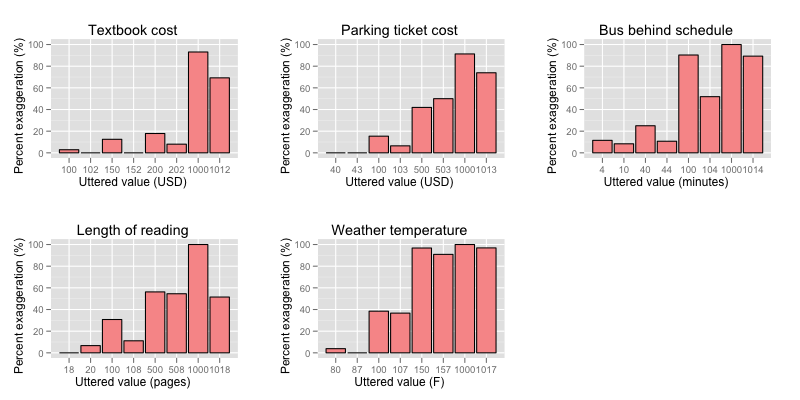
\includegraphics{halo_all.png}}
\caption{Percentage of subjects who judged the utterance to be hyperbolic given an uttered price.}
\end{figure}

Consistent with our predictions, results showed that the proportion of subjects who perceived the utterance as hyperbolic varied as a function of both the distance between uttered and expected price as well as the ``roundness" of the uttered price. As shown in Figure 4, subjects were more likely to judge an utterance as hyperbolic as the uttered price moved further away from the expected price. However, subjects' responses also demonstrated a pragmatic halo effect. Figure 5 illustrates these two effects and their interaction more clearly. The top graph in Figure 5 plots the distance of the uttered price from the mean. This explains why few subjects perceived the utterance as hyperbolic when the uttered price was \texttt{100}, which was very close to the mean, while many subjects perceived the utterance as hyperbolic when the uttered price was \texttt{1000}, which was very far from the mean. The bottom graph in Figure 3 plots the frequency of the numbers used in the uttered prices. The number frequencies were taken from the Google web corpus and approximate how frequently people use certain numbers. We see that these frequencies can explain why fewer subjects perceived the utterance as hyperbolic when the uttered prices were \texttt{243} and \texttt{250} than when the uttered price was \texttt{200}.

\begin{figure}[t]
%\scalebox{0.5}{\includegraphics{combine.png}}
\caption{The top graph plots the distance between the expected price and the uttered price, and the bottom graph plots the frequencies of the numbers in the utterances.}
\end{figure}


We then analyzed how perception of hyperbolic intent and distance between the uttered price and expected price interacted to form subjects' inferences of the actual price. Figure 6 shows the average of subjects' inferred prices given different uttered prices and whether or not they interpreted the utterance as a hyperbole. When subjects perceived a hyperbolic intent, they inferred that the actual price was less than the uttered price and closer to the expected (mean) price. When the uttered price became very unlikely, for example when the uttered price was \texttt{1000}, subjects inferred that the actual price is very close to the mean. When subjects did not perceive a hyperbolic intent, however, they inferred that the actual price was close to the uttered price. 

There are some exceptions and anomalies in this data that we cannot quite explain. For example, if a subject does not perceive the utterance as hyperbolic, then he or she should report that the actual price is identical to the uttered price. However, in the case when the uttered price was \texttt{1000}, some subjects (2 out of 10) responded that it was not a hyperbole, and yet they both reported that the actual price should be $100$. We suspect that some subjects may have misunderstood the question, and since we only had around $10$ subjects for each utterance condition, our data may be noisy and misleading on some points. However, the general trend seems to match our intuitions about how the distance from expected and frequency of number (pragmatic halo) interact in people's interpretation of hyperbole.


\begin{figure}[tl]
%\scalebox{0.44}{\includegraphics{average.png}}
\caption{Average inferred price participants reported given an uttered price.}
\end{figure}


\section{Comparison and Discussion}
Our model captures some important intuitions regarding the numerical values and statistical properties of the uttered price. Here we compare our model results and behavioral data on two aspects: (1) Probability of interpreting the utterance as hyperbolic (2) Most likely inferred price given that the utterance is interpreted as hyperbolic or literal.

\begin{figure}[tl]
%\scalebox{0.46}{\includegraphics{comp_intent.png}}
\caption{Probability that model or human interprets the utterance as hyperbolic}
\end{figure}

As shown in Figure 7, the probability that the model interprets the utterance as hyperbolic roughly matches that of the behavioral data, at least in the general trend. It appears that humans are less affected by the actual uttered price and are similarly likely to interpret the utterance as hyperbole when $U = 200$ and when $U = 1000$.

\begin{figure}[tl]
%\scalebox{0.46}{\includegraphics{no_intent.png}}
\caption{Comparison of model and human inferred price when listener interprets utterance literally}
\end{figure}

Figure 8 shows the model and humans' inferred prices when there is no perceived hyperbolic intent. Since the model and participants alike interpret the utterance literally and believe that $A = U$, the model predictions almost perfectly match the human responses. Interestingly, the model and humans also infer a similar price when $U = 1000$. Our model infers a value of close to $100$ even when it detects no hyperbolic intent, because the prior probability $P(A = 1000, O = \text{no opinion})$ is extremely low. We are not sure why humans also have this interpretation, although it would  be interesting to examine and verify with further data.

\begin{figure}[tl]
%\scalebox{0.46}{\includegraphics{has_intent.png}}
\caption{Comparison of model and human inferred price when listener interprets utterance as hyperbolic}
\end{figure}

Figure 9 shows the model and humans' inferred prices when listener interprets utterance as hyperbolic. We see that there is a fairly good fit when the uttered prices are close to the mean. However, while the model prediction drops close to the mean when $U > 200$, humans' inferred prices follow the uttered prices fairly closely until $U = 1000$. However, since we did not ask humans to make these inferences when $ 250 < U < 1000$, it is unclear if humans' inferred price will also fall back to the mean steadily after a certain threshold price. In general, it appears that human subjects are more willing to believe the speaker. It may also be that Stanford students are more cynical about textbook prices and readily believe in textbooks that cost $250$ dollars.


\section{Future Directions}
Although our model is able to capture the fundamentals of hyperbolic interpretation in this particularly simplistic scenario, more work is needed to extend the model to more complicated settings and generic domains. We would also like to focus on improving the recursive model of a speaker and a listener to better represent the listener's internal model for the speaker, and vice versa. Lastly, our future work will attempt at modeling a speaker's opinion as part of her communicative goals in a conversation, and how a listener can infer the intended meaning.

\section{Acknowledgments}



\bibliographystyle{apacite}

\setlength{\bibleftmargin}{.125in}
\setlength{\bibindent}{-\bibleftmargin}

\bibliography{nips_hyperbole}


\end{document}
